%%%%%%%%%%%%%%%%%%%%%%%%%%%%%%%%%%%%%%%%%%%%%%%%%%%%%%%%%%%%%%%%%%%%%%%%%%%

\documentclass{standalone}

\usepackage{amsmath}
\usepackage{mathptmx}
\usepackage{pgfplots}
\usetikzlibrary{external}
\tikzexternalize{blood-pressure-regression}
\pgfplotsset{compat=1.15}

%% IEEE uses Times Roman font, so we'll default to Times.
%% These three commands make up the entire times.sty package.
\renewcommand{\rmdefault}{ptm}
\renewcommand{\ttdefault}{pcr}
\normalfont\selectfont

\begin{document}

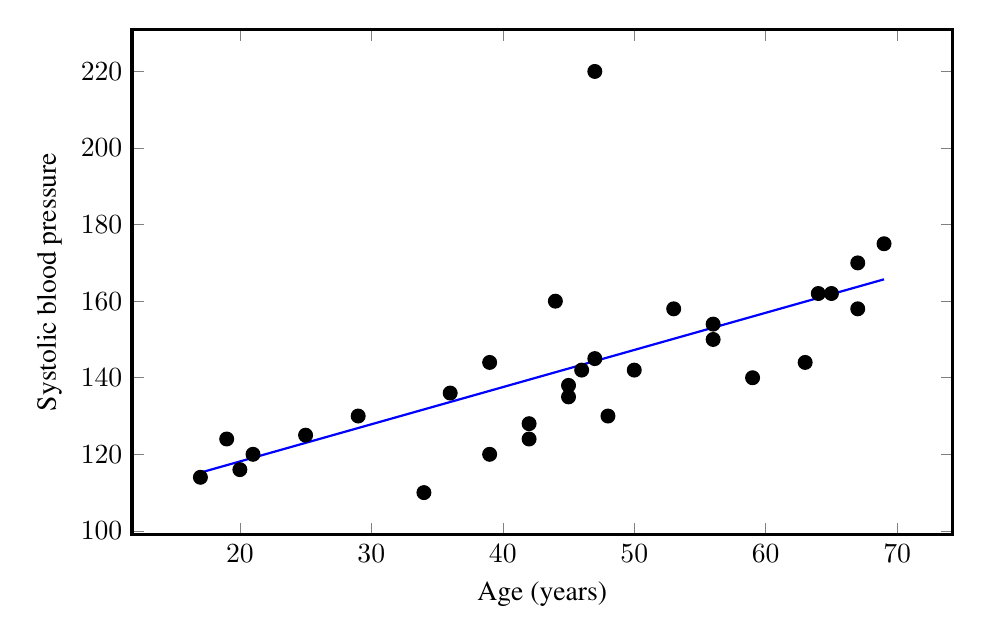
\begin{tikzpicture}
\tikzset{%%
  every mark/.append style={scale=1.0},%%
  scale=1.0%%
}
\pgfplotsset{%%
  every axis/.append style={font=\normalsize}%%
}
%%
\begin{axis}[%%
  axis line style=very thick,%%
  dotStyle/.style={only marks,mark size=2.5,black,mark color=black,mark=*},%%
  enlargelimits=true,%%
  height=8cm,%%
  plotStyle/.style={%%
    domain=17:69,%%
    mark=none,%%
    smooth,%%
    thick%%
  },%%
  width=12cm,%%
  xlabel={\normalsize Age~(years)},%%
  ylabel={\normalsize Systolic blood pressure}%%
]
%%
%%
\addplot+ [plotStyle]
{0.970870*x + 98.714718};
%%
\addplot[dotStyle] coordinates {
  (39,144)
  (47,220)
  (45,138)
  (47,145)
  (65,162)
  (46,142)
  (67,170)
  (42,124)
  (67,158)
  (56,154)
  (64,162)
  (56,150)
  (59,140)
  (34,110)
  (42,128)
  (48,130)
  (45,135)
  (17,114)
  (20,116)
  (19,124)
  (36,136)
  (50,142)
  (39,120)
  (21,120)
  (44,160)
  (53,158)
  (63,144)
  (29,130)
  (25,125)
  (69,175)
};
\end{axis}
\end{tikzpicture}

\end{document}
